\documentclass[11pt]{article}
\usepackage{graphicx}
\usepackage{listings}
\usepackage[margin=1in]{geometry}
\usepackage{placeins}
\usepackage{float}
\lstset{language=python}

\author{Andrew Smith, Kofi Otseidu, Manav Trivedi}
\title{Neural Nets}

\begin{document}
\maketitle

\section{Predicting officer salaries}

We started by creating a table of officer data and salaries from 2017. We specifically only take one year, as including an officers previous years salary probably gives away the current salary, which would make the neural net mostly useless. So we only consider each officer once. The table includes features of rank, race, gender, age, years of service, number of complaints, number of settlements, total amount of settlements, and number of awards. We used one hot encoding for the categorical variables which worked better than simply inputing category codes. The neural net uses 4 dense layers with ReLu activation. The test data has a mean absolute error of \$2017.91, which, for salaries roughly \$50k-180k, isn't bad. We tested a few different configurations but consistently got the best results with the above setup. Looking at the plot of actual vs predicted salaries, it seems to do pretty well with most sections of the spectrum of salaries and there are no clear mismatched areas.

\begin{figure}[h]
\caption{Predicted Salary vs Actual and Error plots}
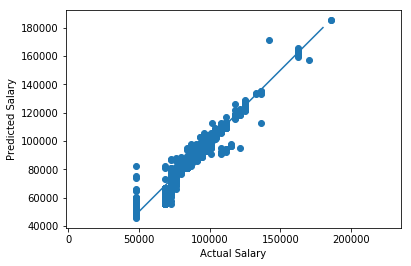
\includegraphics[width=0.5\textwidth]{pred.png}
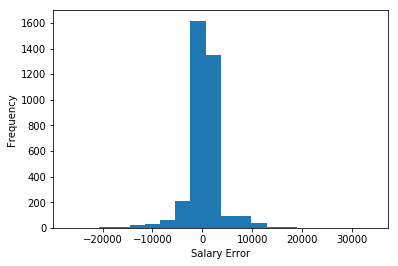
\includegraphics[width=0.5\textwidth]{error.png}
\end{figure}

\noindent Code is as follows:
\begin{lstlisting}
import tensorflow as tf
import pandas as pd
import numpy as np
import matplotlib.pyplot as plt
from tensorflow import keras
from sklearn.model_selection import train_test_split

data = pd.read_csv('neuralnet.csv')
cols = ['rank', 'gender', 'race',
       'current_age', 'years_service', 'salary', 'numAllegations',
       'numSettlements', 'sum_settlement_amount', 'numAwards']
df = data[cols]

#drop null valued rows
df = df.dropna()

#encode categorical values
df['rank'] = df['rank'].astype('category')
df['gender'] = df['gender'].astype('category')
df['race'] = df['race'].astype('category')
df['rank_cat'] = df['rank'].cat.codes
df['gender_cat'] = df['gender'].cat.codes
df['race_cat'] = df['race'].cat.codes

ucols = ['current_age', 'years_service', 'salary', 'numAllegations',
       'numSettlements', 'sum_settlement_amount',
       'numAwards','rank_cat','gender_cat','race_cat']

df = df[ucols]

col = ['current_age', 'years_service', 'numAllegations','numSettlements',
	'sum_settlement_amount', 'numAwards','rank_cat','gender_cat','race_cat']
X = df[col]
y = df['salary']

#normalize data
mean = X.mean(axis=0)
std = X.std(axis=0)
X = (X - mean)/std

#train-test split data
X_train, X_test, y_train, y_test = train_test_split(X,y,test_size=0.3)

#create neural net model
def build_model():
    model = keras.Sequential([
        keras.layers.Dense(128,activation=tf.nn.relu,input_shape=(X_train.shape[1],)),
        keras.layers.Dense(64,activation=tf.nn.relu),
        keras.layers.Dense(32,activation=tf.nn.relu),
        keras.layers.Dense(1)
    ])
    
    model.compile(loss='mse',optimizer='adam',metrics=['mae'])
    
    return model

model = build_model()
model.summary()

#store trained data stats and plot
early_stop = keras.callbacks.EarlyStopping(monitor='val_loss', patience=20)
history = model.fit(X_train, y_train, epochs=500, validation_split=0.3, 
 verbose=0, callbacks=[early_stop])

plt.gcf().clf()
plt.figure()
plt.xlabel('Epoch')
plt.ylabel('Mean Absolute Error')
plt.plot(history.epoch, np.array(history.history['mean_absolute_error']),
       label='Train Loss')
plt.plot(history.epoch, np.array(history.history['val_mean_absolute_error']),
       label = 'Val loss')
plt.legend()
plt.show()

#predict test values and compare
pred = model.predict(X_test)

x = np.linspace(50000,180000,10)
plt.scatter(y_test,pred)
plt.plot(x,x)
plt.xlabel('Actual Salary')
plt.ylabel('Predicted Salary')
plt.axis('equal')
plt.show()

err = pred.flatten() - y_test
plt.hist(err,bins=20)
plt.xlabel('Salary Error')
plt.ylabel('Frequency')
plt.show()

[loss, mae] = model.evaluate(X_test, y_test, verbose=0)
print('Mean Absolute Error = ',mae)
\end{lstlisting}

\end{document}